\section{Introduction}
\label{sec:introduction}

% Motivation
Exploration is a key capability that enables robotic vehicles to operate in
unknown environments. The robot can be controlled to navigate the environment while building a map, leading to traditional simultaneous localization and mapping (SLAM) approaches, as illustrated in Fig.~\ref{fig:ground_bot}. However, this can be extended to also incorporate autonomous path planning, and in this project we develop an active perception policy
for robotic exploration. Active perception exploration formulations
choose control actions which optimize an information-theoretic objective
function such as Shannon's mutual information or entropy
\cite{bourgault2002information, stachniss2005information} over the robot's map,
given a sensor measurement model. Other common exploration techniques, such as frontier
exploration \cite{yamauchi1997frontier}, use geometric reasoning to infer explorative paths.
While these strategies work well in practice, they operate on a
maximum likelihood estimate of the map, and apply heuristics to determine the most uncertain
locations in the environment. In contrast, active perception strategies do not utilize
geometric or maximum likelihood assumptions, and instead interpret the map as a binary
random variable, choosing actions which directly minimize the random variable's uncertainty.
Additionally, information-based exploration methods easily extend to 3D
configuration spaces, a benefit which is not shared by frontier methods.
Julian et al. prove that maximizing mutual information between a
robot's map and expected future map naturally yields explorative behaviors
\cite{julian2013mutual}.

\begin{figure}[t]
  \centering
  \begin{subfigure}{0.47\textwidth}
    \centering
    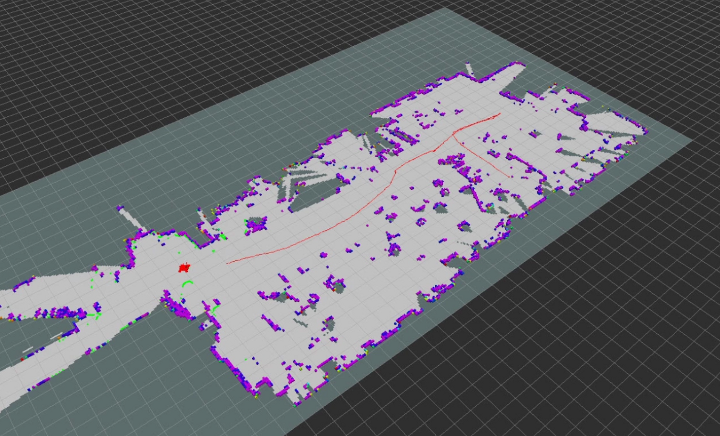
\includegraphics[height=4.3cm]{ground1.png}
    \caption{Map and trajectory\label{fig:ground_bot1}}
  \end{subfigure}
  
  \vspace*{0.1in}
  
  \begin{subfigure}{0.47\textwidth}
    \centering
    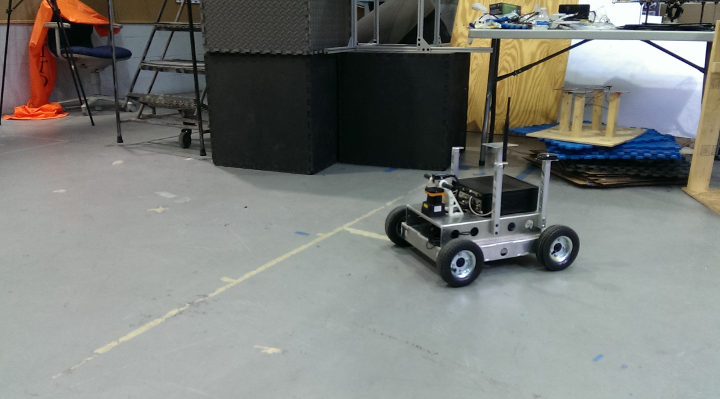
\includegraphics[height=4.3cm]{ground2.png}
    \caption{Ground robot\label{fig:ground_bot2}}
  \end{subfigure}
  \caption{A ground robot mapping while being driven through a cluttered environment.\label{fig:ground_bot}}
\end{figure}

% Overview of our approach
Active perception formulations seek to optimize information-theoretic
objectives. While this optimization is real-time for short planning horizons,
these metrics are often expensive to compute online, requiring double
integration over possible future robot states and measurements, or Monte Carlo sampling
from the distribution of measurements. These expensive per-pose computations inhibit
online dense evaluation over a configuration space. In this project, we aim to develop an
efficient active perception exploration strategy which evaluates the
information-theoretic objective in a sparse, but well-chosen set of poses across the
configuration space. This strategy evaluates the objective function
a limited number of times, while still generating paths that sufficiently explore the space.

% Overview of RRT
To achieve real-time active perception exploration, we use a Rapidly-Exploring Random Tree
(RRT) to generate sets of dynamically feasible actions over a finite planning horizon
\cite{Kuwata09_TCST}. RRT planners trade trajectory optimality for efficiency, allowing for evaluation
of many potential future locations in the configuration space during a single planning
step. In addition, RRT planners are anytime, and generate potential trajectories
for a pre-specified amount of time before evaluating the most optimal sampled trajectory. Our
strategy evaluates each RRT leaf-node using the information-theoretic objective function,
and stores the resulting reward in the tree. After planning for a specified
amount of time, the maximum reward leaf-node is chosen as the optimal location to
visit, and the RRT is traversed to generate a dynamically feasible trajectory to
that location.

% Overview of CSQMI
In addition to the efficiency gains from using an RRT, a recent work by Charrow
et al. \cite{charrow15} has
proposed the Cauchy-Schwarz Quadratic Mutual Information (CSQMI) as an efficient
information-theoretic objective function. CSQMI is theoretically
well-motivated: it is derived from Renyi's Quadratic Entropy, a generalization of Shannon's entropy.
However, in contrast to Shannon's mutual information (which is derived directly
from Shannon's entropy), CSQMI is shown to have superior computational efficiency.

% Results and implementation
The contribution of this work is an exploration framework to enable online exploration using CSQMI in sparse
planning graphs, such as RRTs. 
We discuss the
formulation and implementation of the CSQMI metric, RRT, and an Unscented Kalman Filter (UKF) that were developed to enable trajectory tracking and
state estimation.
Finally, we demonstrate the performance of our approach
through a set of simulations in which a mobile ground
robot must explore an unknown space using a laser scanner range sensor.

% Overview of sections
This paper is structured in the following manner: Section~\ref{sec:occupancy_grid_mapping}
gives a brief overview of occupancy grid mapping which is necessary for the CSQMI
information metric. Section~\ref{sec:information_theoretic_objective}
details the CSQMI information-theoretic cost objective and its similarities to
Shannon's mutual information. Section~\ref{sec:measurement_model} discusses the
measurement model that was chosen to evaluate expected future measurements.
Sections~\ref{sec:planner} and~\ref{sec:state_estimation} cover the RRT and UKF formulations
used in our implementation. Finally, Sections~\ref{sec:results}
and~\ref{sec:conclusion} give results and analysis of our implementation in
simulation, and describe future work towards implementing our algorithms on a
ground robot.
